\documentclass[11pt]{article}
\usepackage[utf8]{inputenc}
\usepackage{geometry}
\geometry{a4paper, margin=1in}
\usepackage{enumitem}
\usepackage{hyperref}
\usepackage{tikz}
\usetikzlibrary{positioning, arrows.meta}

\title{\textbf{Project Report: ``The Compliance Clerk'' - Intelligent Document Extraction}}
\author{\textbf{Author:} Yashpal Yadav \\ \textbf{Project:} The Compliance Clerk (Hiring Assignment)}
\date{}

\begin{document}

\maketitle

\section{Executive Summary}
This report details the design, architecture, and implementation of \textbf{The Compliance Clerk}, an automated document extraction pipeline. The system was developed to replace slow, error-prone manual parsing of heterogeneous government documents---specifically Traffic eChallans and Non-Agricultural (NA) Permission PDFs. By leveraging an advanced OCR fallback strategy coupled with Large Language Model (LLM) function calling, the tool ingests unstructured PDFs and securely transforms them into structured, queryable Excel reports. This automation provides immediate value to operations teams by significantly reducing processing time, minimizing human error, and ensuring compliance through an immutable audit trail.

\section{System Architecture \& Pipeline}

\begin{center}
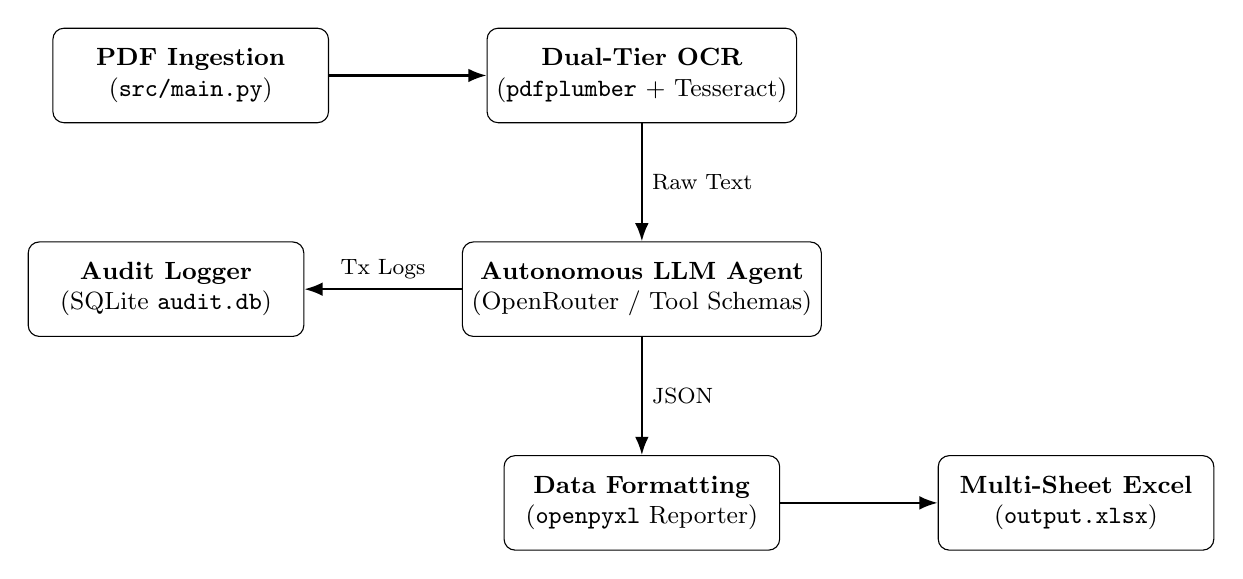
\begin{tikzpicture}[
  node distance=1.5cm and 2cm,
  box/.style={draw, rectangle, align=center, minimum width=3.5cm, minimum height=1.2cm, rounded corners, font=\small},
  arrow/.style={-Latex, thick}
]

% Nodes
\node[box] (input) {\textbf{PDF Ingestion}\\(\texttt{src/main.py})};
\node[box, right=of input] (ocr) {\textbf{Dual-Tier OCR}\\(\texttt{pdfplumber} + Tesseract)};
\node[box, below=of ocr] (agent) {\textbf{Autonomous LLM Agent}\\(OpenRouter / Tool Schemas)};
\node[box, left=of agent] (audit) {\textbf{Audit Logger}\\(SQLite \texttt{audit.db})};
\node[box, below=of agent] (reporter) {\textbf{Data Formatting}\\(\texttt{openpyxl} Reporter)};
\node[box, right=of reporter] (output) {\textbf{Multi-Sheet Excel}\\(\texttt{output.xlsx})};

% Lines
\draw[arrow] (input) -- (ocr);
\draw[arrow] (ocr) -- node[right, font=\footnotesize] {Raw Text} (agent);
\draw[arrow] (agent) -- node[above, font=\footnotesize] {Tx Logs} (audit);
\draw[arrow] (agent) -- node[right, font=\footnotesize] {JSON} (reporter);
\draw[arrow] (reporter) -- (output);

\end{tikzpicture}
\end{center}

The document processing pipeline operates as a linear, fault-tolerant state machine:
\begin{enumerate}[label=\arabic*.]
    \item \textbf{PDF Ingestion \& Routing:} The orchestrator (\texttt{src/main.py}) safely processes single files or entire directories, routing them into the extraction engine.
    \item \textbf{Dual-Tier OCR Processing (\texttt{src/extractor/}):} The system primarily relies on zero-loss text extraction using \texttt{pdfplumber}. If the document is an image-based scanned PDF (yielding low character counts), the system automatically rasterizes the pages via \texttt{pdf2image} and applies \texttt{pytesseract} OCR to guarantee text acquisition.
    \item \textbf{LLM Extraction \& Semantic Parsing (\texttt{src/agent/}):} The raw text is passed to an LLM agent connected via OpenRouter (\texttt{qwen3.6-plus:free}). The LLM first classifies the document type, then routes the text into rigid JSON schemas for targeted entity extraction.
    \item \textbf{Structured Data Formatting (\texttt{src/reporter/}):} A dynamic reporter component aggregates the validated JSON payloads and systematically routes the data to distinct, domain-specific sheets (\texttt{eChallan}, \texttt{NA PDF}, \texttt{Lease Deed}) within a formatted \texttt{output.xlsx} file.
\end{enumerate}

\section{Core Implementation Details}

\subsection{Multi-Format Parsing}
To handle diverse document layouts and languages without brittle regex matching, the application relies on LLM semantic understanding. The system successfully extracts:
\begin{itemize}
    \item \textbf{eChallans:} Challan Number, Vehicle Number, Violation Date, Amount, Offence Description, Payment Status.
    \item \textbf{NA PDFs:} Survey Number, Land Area, Owner Name, Order Date, Authority Details.
\end{itemize}
Classification is forced via a preliminary LLM decision step, allowing multi-page or bundled PDFs to be processed conditionally.

\subsection{LLM Integration \& Schema Enforcement}
The core of the LLM integration relies on native \textbf{Function Calling (Tool Use)}. Standard LLM text generation frequently hallucinates JSON structures. To counteract this, \texttt{src/tools/tools.py} defines rigid JSON Schemas representing the exact data models required. By enforcing \texttt{tool\_choice="auto"}, the model is mathematically constrained by the API provider to return structured JSON payloads. This ensures horizontal compatibility when writing to analytical DataFrames/Excel. Context limits are mitigated by utilizing high-capacity models capable of absorbing large OCR dumps.

\subsection{Observability \& Audit Trail}
Given the probabilistic nature of LLMs, the system employs strict observability. An asynchronous transaction logger (\texttt{src/audit/audit.py}) leverages local SQLite (\texttt{audit.db}). Every stage of the interaction---including source file paths, detected document types, explicit tool payloads, raw prompts, API responses, and traceback errors---is persisted. This provides operations and compliance teams with full replayability and a transparent debugging apparatus required for production AI workloads.

\subsection{Version Control \& SDLC}
The project implements a structured software development lifecycle (SDLC) managed via Git. The repository features an atomic commit log demonstrating linear progression: defining OCR infrastructure, wiring the SQLite audit layer, integrating standard API loops, adapting schemas for resilience, and finally formatting the report output. Each commit encapsulates specific features or bug fixes, entirely avoiding massive, monolithic commits in favor of a clean, revertible history.

\section{Technical Challenges \& Solutions}

\begin{itemize}
    \item \textbf{Messy OCR \& Schema Validation Failures (HTTP 400):} 
    \begin{itemize}
        \item \textit{Challenge:} OCR artifacts (e.g., reading ``251/p2'' instead of integer ``251'' for survey numbers) caused downstream validation crashes when the LLM attempted to pass alphanumeric values into strictly typed \texttt{number} fields inside the JSON schema.
        \item \textit{Solution:} Implemented ``Fuzzy Typing'' by relaxing all numeric schema properties to \texttt{string}. This delegated the data-cleaning responsibility safely without instantly crashing the LLM interaction loop, allowing the API to gracefully ingest alphanumeric OCR anomalies and formatting drift.
    \end{itemize}
    
    \item \textbf{Prompt Refinement \& Semantic Overlap:} 
    \begin{itemize}
        \item \textit{Challenge:} The state of Gujarat labels Property Registration and Stamp Duty receipts as ``e-Challans''. The LLM consistently misclassified property documents as traffic violations.
        \item \textit{Solution:} Refined the system prompt to explicitly define the semantic boundary: \textit{``ONLY extract Traffic Violation eChallans using \texttt{extract\_echallan\_fields}. DO NOT use \texttt{extract\_echallan\_fields} for Stamp Duty or Registration Fee receipts.''}
    \end{itemize}
    
    \item \textbf{Rate Limiting \& Throughput:} API endpoint exhaustion was heavily mitigated by migrating the backend LLM provider to OpenRouter and implementing exponential backoffs using the \texttt{tenacity} library to retry queries without data loss.
\end{itemize}

\section{Conclusion}
\textbf{The Compliance Clerk} demonstrates a highly scalable, maintainable, and robust approach to intelligent document extraction. By decoupling the OCR ingestion, LLM schema enforcement, audit logging, and reporting layers (Separation of Concerns), the codebase acts as a reliable foundation. The strict tool-calling schemas ensure data integrity, while the localized SQLite audit trails guarantee transparency. The architecture is ready to scale seamlessly; adapting to new document types requires simply passing new JSON schemas, proving its design as a robust enterprise grading submission.

\end{document}